\documentclass[11pt]{article}

\usepackage[hyphens]{url}
\usepackage[implicit=true,%
            bookmarks=false,%
            bookmarksopen=false,%
            pdfpagemode=UseNone,%
            pageanchor=false,
            colorlinks=false,%
            pdfborder={0 0 0},%
            plainpages=false,%
            pdfpagelabels=true,%
            pdfpagelayout=SinglePage]{hyperref}
\usepackage[sort&compress,numbers]{natbib}
\usepackage{skull}
\usepackage{ragged2e}
\usepackage{fancyhdr}
\usepackage{xspace}
\usepackage{fullpage}
\usepackage{graphicx}
\usepackage[capitalize,sort&compress]{cleveref}
\usepackage{mathptmx}
\usepackage[scaled=0.83]{berasans}
\usepackage[scaled=0.83]{beramono}
\usepackage[colorinlistoftodos]{todonotes}
\usepackage{alltt}
\usepackage[OMS,OML,T1]{fontenc}
\usepackage{textcomp}
\usepackage{caption}
\usepackage{subcaption}
\usepackage{paralist}

\renewcommand{\bfdefault}{b} % used to eliminate most
\renewcommand{\sldefault}{it} % "font not found" warnings
\usepackage{tikz}
\usetikzlibrary[backgrounds,calc,positioning]
\usepackage{enumitem}

\begin{document}

\setcounter{page}{1}
\pagestyle{empty}
\hypersetup{pageanchor=false}

\begin{center}
{\Large By the People, For the People:\\
  Community Ratings for App Privacy}
\end{center}

\smallskip

\centerline{\bf }

\bigskip

\pagestyle{plain}

\section{Introduction}

Apps---third-party programs with a clean installation model and
restricted permissions---have become ubiquitous 
\cite{gplay-50-billion, apple-50-billion}.
The app model is most commonly associated with smartphones, 
such as iPhones and Android handsets. However, the model now has much 
wider adoption. Apps now appear in a variety of domains,
such as tablets, browsers (in the form of extensions), PC operating 
systems, smartwatches (such as the Pebble), 
home automation (like Microsoft's HomeOS \cite{ms-homeos}),
and cars (such as \emph{iOS in the Car} \cite{cars-apple} and Android's 
partnership with Audi, GM, and Honda \cite{cars-google}).
Most app ecosystems are also supported by a ``store'' or
``marketplace''---a central repository that
enables users to search for, browse,
investigate, and install apps on their devices. 

Apps and app stores allow users of a broad range
of technical ability to customize their devices.
However,  
because of the amount of user information associated with these 
devices, installing third-party apps presents 
risks to user security and privacy. 
%\cite{android-repackaged-CODASPY12}
%http://www.esecurityplanet.com/views/article.php/3928646/Top-10-Android-Security-Risks.htm
%Esecurity blog post discussing the top ten risks to Android user
Some of these risks are malware apps, or apps that highjack
over-provisioned apps to perform malicious operations. This is a topic
of extensive research 
\cite{droidrisk-2013, android-repackaged-CODASPY12, comDroid-MOBISYS11}, 
but does not address a different,
important problem: \emph{how to help users make informed privacy and
  security decisions about apps based on the permissions that the apps
  demand}.

The permission models and their presentation vary across manufacturers
(Fig.~\ref{permsOSs} shows iOS, Windows 8, and Android). Android and
Windows take a ``static'' approach, in that apps are given a
\emph{manifest} of
permissions at installation time, and may use any of them at will at runtime. In
Android, users explicitly approve these during the installation
process; Windows lacks an approval step (permissions are listed on the
app's page in the marketplace, and consent is presumably assumed when
the user installs the app). In contrast, iOS uses a ``dynamic''
approach: permissions are not listed explicitly; instead, users must
approve access to permissions when an app tries to use them.

\begin{figure*}[ht]
\centering
    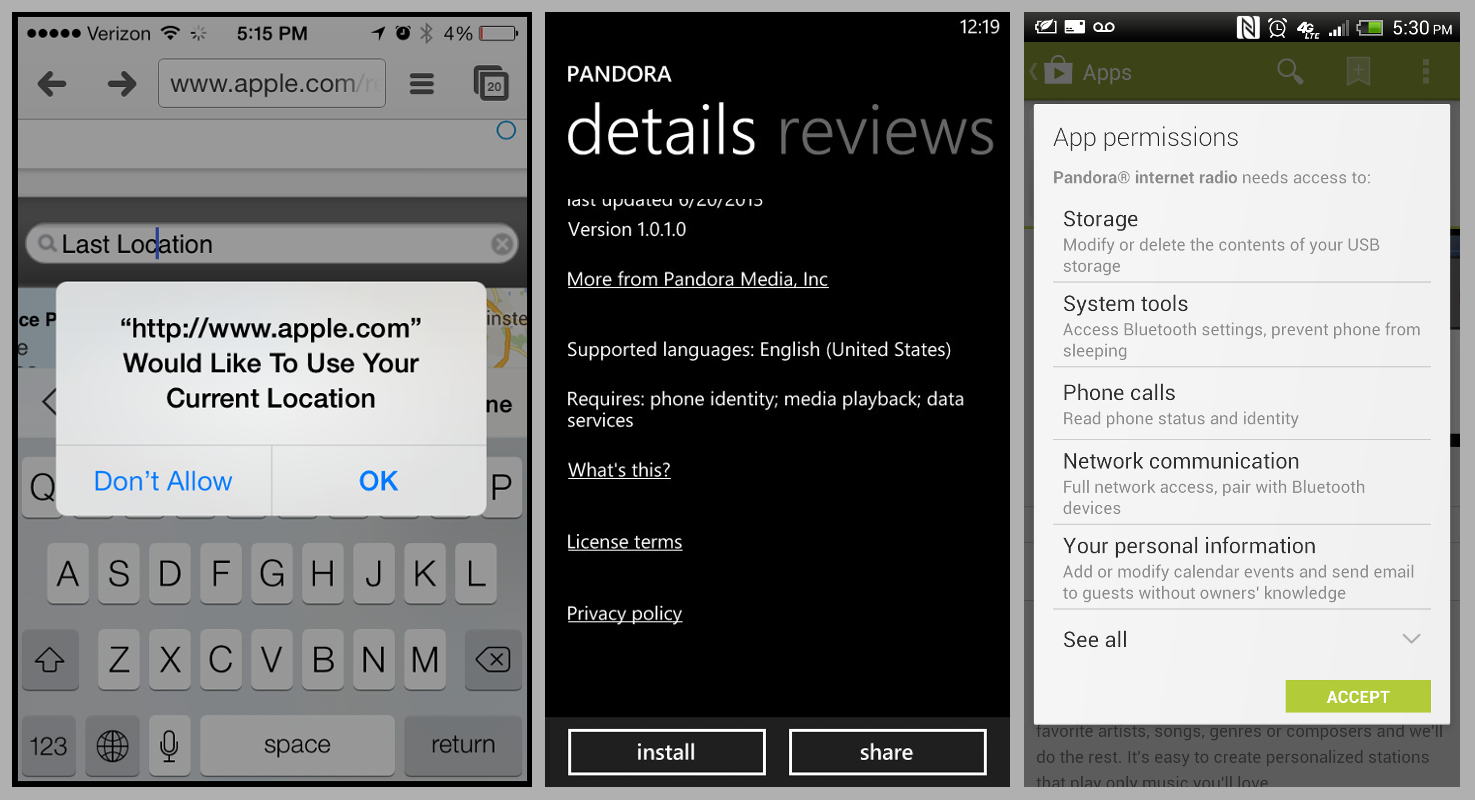
\includegraphics[width=\linewidth]{img/OSscreenshots.png}
    \vspace{1pt}
    \caption{The presentation of permission information on iOS, Windows, 
    and Android, from left to right}
    \label{permsOSs}
\end{figure*}

There are advantages and disadvantages to each approach. Nevertheless,
this proposal falls firmly in the static model. For one thing, only by
seeing all permissions can users reason about their potential
combinations. More importantly, we believe that asking for permissions
during execution will often result in consent that might not otherwise
have been given, because users are likely to grant whatever appears
necessary to complete a task \cite{phisher-wanings-SIGCHI08}. In contrast, the static
model---especially if combined with the ability to turn off individual
permissions (discussed in Sec~\ref{subsubsec-perm-man-asst})---in 
principle enables a more contemplative and
informed approach to choosing apps based on permissions.

Unfortunately, current practice seems to fall short of this principle
in numerous ways.  Many users are uninformed about the suitability of
an app's permissions, and have no clear means to learn more about
their suitability. For users who do
believe a permission is unnecessary, there is no structured method to
communicate their view---comments to this effect are often found in
the ratings of apps, but these comments can be difficult for other
users (especially uninformed ones who would like guidance), and even
developers, to find. In turn, developers have no structured way to
respond to such comments and justify their apps'
needs.\footnote{Sometimes, seemingly unnecessary permissions can
  appear to have justifications. For instance, the PI communicated
  with the developers of Dropbox, asking why it needed ``Phone calls
  -- read phone state and identity''. Their response was, ``[T]he
  phone state \& identity is simply because we need a unique ID for
  each cell phone, so we use the IMEI to keep track of phone/user
  combinations.'' This arguably points to a weakness of the Android
  APIs, which others have noted \cite{effectivness-perms-USENIX11}.} Finally, this entire problem
is greatly exacerbated by continuously growing manifests.

When expressed loudly and emphatically, user opinion about privacy can
sway developers. A recent incident with Avis illustrates a (sadly,
rare) success. Avis added ``List of Running Apps'' to the permissions
required by their Android app. Users protested the change in the
reviews, with numerous comments like, ``I refuse to update and will
likely uninstall until you can justify the need to access my `Running
Apps'.'' In response to the backlash, Avis removed the offending
permission, and the newest version of their app (as of January 2,
2014) does not require it. Avis states on their app's Google Play
page:
\begin{quote}
  We've updated the permissions in this version to not require List of
  Running Apps. We had that in place to help analyze and improve app
  performance, but removed it due to your voiced concerns.
\end{quote}

Our goal is to make such successes commonplace. We intend to leverage
the willingness people already demonstrate to provide ratings, and
their familiarity with mechanisms like rating systems, by building systems to rate
\emph{permissions}. These ratings then serve as a guidepost to other
users as they choose which apps to install. 
Indeed, the ratings can be used to \emph{rank} apps
so that more privacy-sensitive apps are rewarded by appearing higher,
while questionable ones percolate down in the list. In turn, a
permission-rating app interface becomes a channel for developers to
convey their needs and intent back to users, thereby enabling more
informed decisions. The feedback of developers also documents their
intent, which can be cross-checked by other tools (e.g., program
analyses).

\section{Preparatory Work}
\label{sec-prep-work}

There are multiple ways to deploy user ratings of permissions. One is
through an app store that uses these ratings to sort
apps. The other is through an app that helps users decide
which individual permissions to turn on and off. We discuss these
models in more detail in Sec~\ref{subsec-the-apps}.

In order for either model to work, however, it must have user
ratings. This presents a chicken-or-egg problem: In order to get users
to employ systems that show ratings, there must already be present
ratings that offer some value to the user; but users would have to be
using a rating app already in order for it to collect user
ratings. We therefore wanted to know if there was another way to
acquire ratings for the marketplace.

Because we would prefer to have a large number of ratings,
crowdsourcing seemed a natural fit. However, crowdsourcing via
platforms like Mechanical Turk also raises various concerns. Will
reviewers take the rating task seriously? Will they give ratings that
are actually distinct enough to reveal differences? Will they rate the
permissions contextually? This last point is subtle: permissions are
not inherently ``good'' or ``bad'', but acquire meaning in the context
of the app's intended purpose.\footnote{For example, we
  downloaded an app that helped turn on and off individual permissions
  on the basis of perceived threat. However, the threat was not
  specific to the app. Thus, on the very first app we examined---that
  for Google+---the permission marked as most dangerous was that to
  share to social streams\dots which is the very point of the app.}

Based on these concerns, we did a series of preliminary studies designed to answer
these questions:
\begin{itemize}
\item Could we gather a large number of conscientious ratings through crowdsourcing?
\item Would those ratings be useful?
\item What are some factors that might affect how users perceive and rate 
app permissions?
\end{itemize}
We deployed a series of studies on Amazon's Mechanical Turk. We chose
Mechanical Turk because it can be very cost effective, and has become
a common platform for academic research, which gave us guides of how
to best use it \cite{reseach-mturk-BRM12, mturk-data-quality-PPS11}. 
Our study presented users with surveys that
described an app, preceded by a motivating paragraph asking
them to imagine that they came by this app in some way and needed an
app of that functionality.  We used fourteen apps: Facebook, GMail,
Pandora, Angry Birds and ten weather apps.  The descriptions
of the apps were taken from their Google Play pages, including the
permission information. Given this information, users were asked
whether they would download the app, and to rate each of the app's
permissions as either ``acceptable'' or ``unacceptable,'' and were
given an optional text box to explain each of their ratings.

Once we had workers completing tasks, we needed to ensure that the
users were real humans who were actually answering the questions we
asked. We manually reviewed the responses in the optional text boxes
that allowed users to explain their ratings. Overall, we found that
users did provide explanations for their ratings despite this being
optional. Furthermore, their responses were relevant to the
permissions being discussed, indicating that the responses were from
real people thinking about the task. Because these were preliminary
studies, we did not do any significant analysis on the text answers,
but we will in proposed work. Additionally, we will want to further
validate our Mechanical Turk results by comparing them with results
from other populations. There are also other measures we will want to
use to increase confidence in our Mechanical Turk data, such as test
questions.  We discuss all this in Sec~\ref{sec-eval}.

\begin{figure*}[t]
\centering
    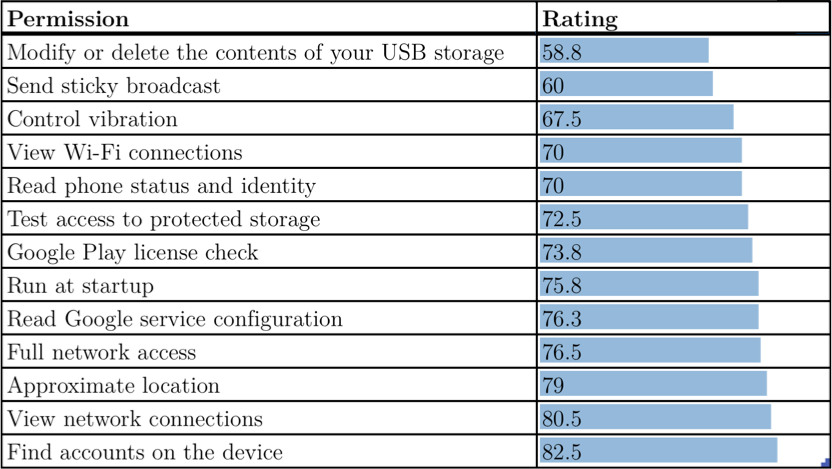
\includegraphics[width=.6\linewidth]{img/RatingTable.png}
    \vspace{1pt}
    \caption{The range of approval ratings for the permissions from the 
    weather apps surveyed}
    \label{weatherratings}
\end{figure*}

Next, we looked for variations in ratings between permissions. To
compare within a domain, we focused on the weather apps. Across the
ten apps, a total of thirteen permissions were used. These were rated
as shown in Fig.~\ref{weatherratings}.  Although the approval rate for
every permission was over 50\%, approval varied from 58.8\% to
82.5\%. This range of ratings suggests that users were actually
distinguishing between the permissions (not treating them all
uniformly, which might be another indication of not taking the rating
task seriously or not understanding it); we also found correspondence
between their ratings and their textual comments.

To answer our third question, we looked only at Facebook, Gmail,
Pandora, and Angry Birds.  We used these same basic surveys, but
varied specific conditions in the survey. The conditions we created
were: asking the user if they would download the app before or after
they were asked to rate the permissions; how the user discovered the
app (on recommendation from a colleague, because it was a featured app in
the app store, or because it was highly rated in the app store); and
whether the app was ``brand-name'' or generic. To create the generic
apps, we reused the Play Store descriptions of the apps but replaced all
instances of the app's name with a generic name. For example, GMail
became MongogoMail.  Additionally, we changed any obvious identifiers,
so the pigs and birds from Angry Birds became warriors and invaders.

Varying where users were asked whether they would download the app (either before or after rating the permissions) was
meant to investigate whether users were more or less likely to
download an app if they had been primed to think about privacy by
rating the permissions. We found that there was no significant change
in either the percentage of users who would download the apps, or the
ratings the provided.

Varying how the user was asked to imagine they discovered the app
could affect their opinion of the permissions, or their willingness to
download the app. In this case, only Facebook showed any interesting
results: respondents were less likely to install the app if it
had been recommended by a colleague than if it was featured or highly
rated. We found this result is odd given that, due to the network
effect of an app like Facebook, we would expect the app to be more
valuable if friends or colleagues also use it. However, it did not
seem to be a pervasive effect.

Varying branding did not have a significant effect on downloads or
ratings for Pandora and Angry Birds, but did 
for GMail and Facebook. In both cases,
participants rated the generic version's permissions as less
acceptable. However, for GMail, a lower percentage of users said they
would install the app, but this was not true of Facebook.  These
findings suggest that branding may be an important part of users'
feelings about an app. However, these results also raise questions
about how privacy and functionality interact in user decisions. Are
people less approving of these generic apps because they think they
are unsafe, or because they feel they will not have access to their
existing email and social network accounts?

To separate access concerns from privacy concerns, we did a follow-up
study asking subjects to evaluate an app that was an
interface over a brand-name app. For instance,
subjects were presented with Gmore!, an app purporting to offer a
smoother interaction with one's GMail account. Again, subjects rated
the off-brand apps' permissions as less acceptable, and again, a lower
percentage of users said they would use Gmore!. This suggests that
subjects were concerned about the privacy of the apps, not just their
functionality.

Our preliminary studies suggest that we will be able to gather
meaningful ratings from Mechanical Turk. We believe this is vital
to seed data in a privacy-centric marketplace, and hence attract users
to it. Further, our early examination of these ratings 
suggests insights into how users think about their privacy, and reveals
factors that affect their opinions. These insights may be useful for
further development of our marketplace, and may also be more broadly
useful to the privacy research community.

\section{Proposed Work}

We intend to gather user ratings of app permissions, create apps to present these ratings
to users (and obtain new ratings from them), and study factors that
affect how people perceive the reasonableness of permissions in
different apps. Our primary means of disseminating ratings will be
a pair of apps, both of which will incorporate the ratings we
garner. One app will use permission ratings as a means for sorting
apps (thereby giving priority to the least offensive apps),
while the other will help users turn individual permissions on and
off. We discuss these apps in Sec~\ref{subsec-the-apps} and focus on 
their user interface in Sec~\ref{subsec-perm-ui}. In Sec~\ref{subsec-gather-ratings} 
we discuss our plans to obtain ratings at scale. In
Sec~\ref{subsec-app-selection} we talk about avenues for personalization, and in
Sec~\ref{subsec-analyzing-ratings} propose
some more speculative research.  We discuss evaluation of all these
proposals in Sec~\ref{sec-eval}.

\subsection{The Apps}
\label{subsec-the-apps}

The primary goal of our proposed work is to give end users better tools to make decisions
about their privacy. We will do this directly by building and app, designed for the Android 
operating system, that can be installed 
and utilized by end users. We choose to build atop Android for two reasons.
First, Android is a widely use operating system: according to Nielsen 
\cite{android-market-share}, a consumer research 
company, as of August, 2013, 52\% of smartphones in the United
States use Android, and its penetration in some other countries is
even higher.
Secondly, the Android permission model forces apps to explicitly state which permissions
they require to run, which allows us to programmatically extract the permissions for each 
app, making it much easier to evaluate the permissions. 

\paragraph{The Privacy-Aware App Marketplace}
\label{subsubsec-privacy-store}

An app store offers users a way to search, examine, and download
apps.  Google Play, the built-in store for Android, gives
users access to over a million apps, and allows users to search by
popularity and functionality rating. Unfortunately, there is no way to incorporate
permission information in to the search. We believe this hinders the
user's ability to find privacy-conscious apps, because they have to
look at the permissions for each app they are considering, and are
heavily biased by the app \emph{quality} ratings (stars), which may
have little correlation with permission-sensitivity. Our marketplace
will allow users to search by privacy criteria instead: in other
words, we will construct an app store that sorts apps primarily by
quality but secondarily by privacy-sensitivity, so that the best apps
\emph{that are also rated as requiring the most reasonable
  permissions} appear first.

Google Play does try to inform users about permissions by offering a
brief explanation of what each permission does. However, these
explanations are not specific to the app, and so do not help
users understand how the app might be using the permission. We
believe this is an important factor, because in many cases a
permission that is perfectly legitimate for one app might be cause for
alarm in another. For example, location information makes lots of
sense for a weather app, but (absent other explanation) seems much
more suspicious for a flashlight app. In contrast, our app will
provide user ratings of each permission for each app (with, on demand,
comments), as well as any responses or clarifications provided by the
developers. Because these ratings are specific to the app, we believe
they will enable users to arrive at an \emph{informed} decision about
the permissions each app seeks.

As added justification for this app, Felt et al.\ \cite{android-attention-SOUPS12} 
found that only 17\% of users surveyed looked at the permissions during
their last installation. The authors suggest that the timing of
permission presentation could contribute to the lack of attention paid
to the permissions, because it seems to encourage users to click
through the permissions to complete their task in much the same way
that pop-up warnings do. We believe that sorting apps by permissions
significantly ameliorates this problem, because sorting by permissions
means permissions have been significantly accounted for \emph{before}
users are required to make installation decisions.

To lift ratings from an individual permission to an entire app
requires some method of aggregation. In 
Sec.~\ref{subsubsec-personalizing}, we propose that users
can establish personal privacy profiles, which would effectively offer
weights by which the permission ratings can be combined. Absent that, we will design a
number of possible composition methods. One solution is to simply take
an average over the individual permission ratings. Other options would
be a sparklines-style composition where users could visually see the
general level approval of an apps permissions, or allowing the
community to rate the permissions that are most important for an app.

It should be noted here that regardless of whether users of the
marketplace are seeing ratings from Mechanical Turk workers or other
users, the app should make clear that these are community ratings, not
ratings provided by experts or the developers of the marketplace.


\subsection{The Permission User Interface}
\label{subsec-perm-ui}

Because our goal is to communicate privacy information to users, the
interface used to present permissions will be a critical component of
our work. We want users to be able to make privacy decisions with a
minimum of cognitive effort. Therefore, the interface must display community
ratings to users in an easily understandable way, and should help
users understand the gravity of a negative privacy rating. The
interface must also be usable, allowing users to navigate and use its
features easily. Fig.~\ref{test-UIs} shows mockups of what such
interfaces might look like. Each interface employs UI elements to try
to help
users understand which permissions have positive privacy
ratings and which have negative ratings.

\begin{figure}
\centering
\begin{subfigure}{.5\textwidth}
  \centering
  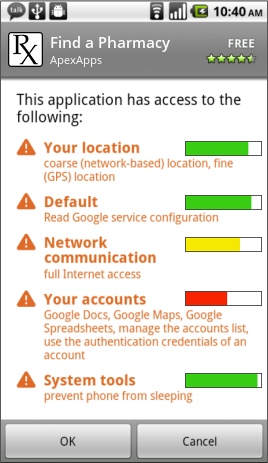
\includegraphics[width=.65\linewidth]{img/PercPerms.png}
  \label{perc-perms}
\end{subfigure}%
\begin{subfigure}{.5\textwidth}
  \centering
  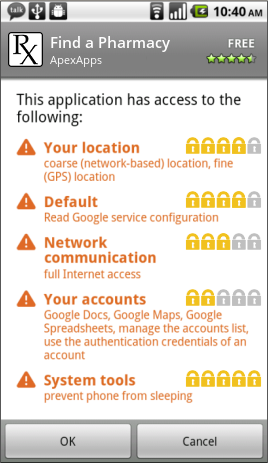
\includegraphics[width=.65\linewidth]{img/LockPerms.png}
  \label{locks-perms}
\end{subfigure}
\vspace{1pt}
\caption{Examples of potential interfaces for a privacy-conscious app marketplace}
\label{test-UIs}
\end{figure}

 
The current Google Play interface attempts to help users in making
privacy conscious decisions by presenting the permissions to the user
and requiring the user to approve the permissions before
proceeding, but we feel this is insufficient in helping users to make informed decisions. In Sec~\ref{subsubsec-privacy-store}, we discuss some 
studies that criticize its
current utility.

An ideal interface should have a few important characteristics:
\begin{itemize}

\item
It should be \emph{intuitive}. That is, even without training, users
should be able to guess the purpose of the interface. We will study a
variety of visual icons---locks, eyes, ``Anonymous'' masks, stars,
bars, etc.---to identify which best suggest the purpose of our apps.

\item
It should suggest \emph{caution}. Permissions that are rated as more
dangerous should be perceived as more dangerous. The use of color and
number or width of icons is likely to be useful here.

\item It should \emph{not mislead}. A ``less negative'' rating is not
  at all the same as a ``positive'' rating. The left interface in
  Fig.~\ref{test-UIs} is potentially bad in this regard because the
  use of green might suggest that the permission has been rated as
  ``good'': a wide green bar might suggest that people are
  \emph{strongly encouraged} to accept this permission, whereas its
  intended meaning is that they are \emph{somewhat discouraged} from
  doing so.

\end{itemize}

We will test the user interfaces by posting survey tasks on Mechanical
Turk. This will allow us to gather a large number of responses in a
cost effective way. Buhrmester et al.\ \cite{mturk-data-quality-PPS11} show that data from Mechanical
Turk are reliable compared to data from more traditional
methods. Additionally, Mechanical Turk offers options to improve the
reliability of workers. We will require workers with a lifetime
approval rating of 97\%, who have done at least 500
tasks. 

Additionally, we will perform in-person studies, such as interface
walkthroughs, with subjects drawn from a university and general city
population, as we discuss in Sec~\ref{para-eval-ui}.


\subsection{Gathering User Ratings}
\label{subsec-gather-ratings}

Ideally, the users of our systems will provide ratings for
apps. However, 
to bootstrap our systems, we will use Mechanical Turk to gather
ratings. Based on several experiments, we find that we can obtain
quality ratings for no more than \$0.30 per worker. Since about thirty
ratings give us sufficiently strong reviews, we can rate each
app for no more than \$10. We have therefore budgeted money to
seed the store with ratings, both for the most popular apps overall,
and for the most popular apps in select categories that people are
likely to search for (e.g., weather, finance, etc.).

This bootstrapping processes uses an ``offline'' model, in that we
will accumulate these ratings so as to seed our apps before anyone
sees them. In principle, however, these ratings could also be done
``online'': that is, if a user is interested in a particular area, or
even a particular app, they could request ratings, spawning fresh tasks for
generating ratings on demand. The speed at which a user gets reviews
depends on number of variables, such as the time of day and day of
week, but we believe the most important variable---based on our
experiments---is how much one is willing to pay for reviews. We
therefore intend to post a series of tasks, staggered by time and
cost, to construct an approximate valuation curve that indicates how
much one needs to pay in return for obtaining quality reviews within a
particular duration of time. In principle, this curve is a function
that can be passed on to the user, who can decide how much they are
willing to spend in return for how long they are willing to wait for
reviews to be completed for their task.

In general, ratings will only be useful if they come from users with some
familiarity with the app models.
In our preparatory studies, we did not validate that respondents are
smartphone users (other than in the task description). In future
studies, we should ask users a test question such as what operating
system version they use on their device. Users could, of course, lie
about this, but it may help us to catch users who simply did not read
our requirements.

\subsection{App Selection: Putting the Ratings to Work}
\label{subsec-app-selection}

The permission ratings may be useful in helping users to choose apps, but
they could be used to improve the user's privacy in other ways as well. They could
also be useful to developers in understanding how users perceive their apps 
and improve their apps based on that feedback.

\paragraph{Personalizing the Marketplace}
\label{subsubsec-personalizing}

The privacy ratings are meant to help users make decision about whether
an app suits their specific privacy needs. Because each user will have a different
set of privacy concerns, the store would be more useful if it was personalized
to each user.

Building privacy profiles for each user would allow users to see ratings from
others with similar privacy concerns. Privacy profiles could be built either by 
analyzing the reviews a user leaves, or by explicitly surveying them about their
privacy concerns. 

In addition to ratings from people with similar concerns, users may want to get
ratings from people they trust. Allowing people to build off of their existing 
social networks could give them greater confidence in the ratings. If users 
establish an account within the marketplace, they could designate other trusted
users, and choose to see reviews only from those users.
These other users could be trusted friends or family with stronger
computing or security knowledge (a stereotypical example of this is a
young adult helping their less comfortable parents or grandparents with technology).

\subsection{Analyzing Privacy Ratings}
\label{subsec-analyzing-ratings}

The user ratings of app permissions will constitute a corpus of 
data about how users think about privacy, and how they use it to make decisions.
Identifying and analyzing trends and patterns in this data may give us 
information that we can use to better understand and meet user privacy needs.

\subsubsection{The Effect of Branding}
\label{subsubsec-branding}

In our preliminary studies (see Sec~\ref{sec-prep-work}), we examined how branding 
affects users' ratings of an app's privacy. We did this by presenting users with
two versions of the apps, one with the brand name, and one with a made-up off-brand
name. We found that for GMail and Facebook, users gave the brand name apps better
ratings, but for Angry Birds and Pandora there was no difference. These results raise
a number of new questions. Why do users care about brand in some cases and not in others?
Do the differences in rating stem solely from privacy concerns, or are users also
considering functionality? These questions may inform developers about how to establish
trust with their users.

We will reproduce our original studies on a larger scale to verify our
preliminary results. Assuming we are able to reproduce our results, we
will examine why users sometimes find the permissions for the
brand name app more acceptable and sometimes do not. To do this, we
will perform the study with a larger set of apps. Our original
study only examined four apps, which does not allow us to
identify characteristics that might influence users ratings. For
example, Facebook and GMail both provide accounts that handle a great
deal of user data. We will therefore include more apps that provide
similar services to see if this effect is common to all those apps.

If we are able to identify common factors that affect user ratings, we
will study why those factors cause the differences in
ratings. Suppose, for example, we were to find that users have a
preference for a brand name in apps that maintain an account, like
GMail. This could because they trust the brand more, or because they
already have an account with the brand, and therefore handing over
more permissions won't do any harm, because they have already given
over much of the information requested by the app.  The specific
questions examined in these studies will depend on our findings from
the first study of branding.

\subsubsection{Communicating With Developers}
\label{subsubsec-dev-comm}



\section{Evaluation}
\label{sec-eval}

The primary goal of our work is to help users make informed decisions
about apps based on other users' ratings of app permissions.
Concretely, these ratings will be provided through two Android apps, a
marketplace and a permissions manager. Each of these apps will
depend on a number of components and their interaction. In this
section we will discuss how we will evaluate each of these components.

\paragraph{Seeded User Ratings}

As we have discussed Sec~\ref{subsec-gather-ratings}, we need to seed the system with user
ratings to make it useful from the start. This means acquiring a large
number of user ratings via crowdsourcing. There are two natural
questions to ask about the ratings so obtained: can we obtain them,
and are they any good.

The first question is easy to evaluate: if we can get our desired
number of ratings from Mechanical Turk, we will have succeeded. 

To answer the second question, we need some notion of quality. An
obvious measure is some extrinsic notion of quality, such as agreement
with the ratings of groups of experts. However, this is not
necessarily appropriate: experts, in particular, may have very
different privacy attitudes than general consumers, and disagreement
with experts may simply reflect disagreement about the relative
weighting of privacy factors.

Instead, we believe it is more meaningful to simply incorporate all
reviews \emph{provided they are genuine}. As our preparatory work
Sec~\ref{sec-prep-work} has shown, crowdsourced reviewers do routinely offer responses
that suggest thought and contemplation, even at the level of
individual permissions. It is reasonable to assume that such users are
then taking the rating task seriously, and that their opinions should
be considered fully. Naturally, it is difficult to discern their
seriousness only from checkboxes; in contrast, textual answers provide
a useful window into their attitude towards the task. 

We will therefore generate rubrics to grade responses on whether they
should be included in the app ratings.  The rubrics will be refined
until the researchers show strong intercoder agreement ($\kappa$)
\cite{cohen-kappa-EPM60} when using it.  For instance, we have begun to generate a
rubric for this purpose, applying it to the preparatory work data, and
found high agreement:
\begin{quote}

\begin{description}

\item[Meaningful Rating (M)]

  User's text provides a reason for each rating, and that reason is
  specific to the rating they gave. This may mean an explanation of
  logic, or simply something like ``good'' or ``bad'' corresponding to
  positive or negative ratings. If the user enters the same text for
  every permission, they must demonstrate a very strong understanding
  that the task is about rating permissions. For example, stating that
  they always accept all permissions demonstrates understanding, while
  writing ``good'' or ``safe'' next to each permission does not.

\item[Not Meaningful Rating (N)]

  User did not seem to understand the question, or user enters text
  not related to the permission they are rating. Ratings that just
  describe the functionality of the permission fall in to this
  category.

\item[Cannot Say (C)]

  User did not enter any text answers to support their rating. Users
  who explain all of one type of their ratings (either positive or
  negative) can be counted as meaningful, if those explanations meet
  all the other criteria of a meaningful rating. This requirement is
  mean to catch users who, for example, explain all of their ``no''
  ratings, but do not think that ``yes'' ratings require an
  explanation.

\end{description}

\end{quote}
However, it is unclear that we can automate the application of such
rubrics, and may have to apply them manually instead.

\paragraph{The User Interfaces}
\label{para-eval-ui}

The success of these interfaces depends on the ability of users to
understand and, ideally, use the permission ratings the interfaces provide.

We will evaluate comprehension through user testing. We plan to do
this at two levels: both at scale, through crowdsourced surveys (most
probably through Mechanical Turk), and through in-person surveys,
interviews, and interface walkthroughs such as talk-alouds. The latter
will help us understand nuances of presentation and enable fine-tuning
of the interface, while the former will help determine answers over
larger and broader groups of participants.

In our surveys, especially for crowdsourcing, we will ask users to
explain what they think the ratings are, and ask them questions to
determine how well they understand the interface.  Additionally, users
should be able to understand the ratings at an app level, and
how app ratings correspond with the permission level
ratings. Users should also be able to understand how the ratings could
assist them in making app decisions.

We will also ask users to compare two different app-level ratings. To
determine if users can understand how app-level ratings relate to
permission-level ratings, we will show the user the permission
level ratings alongside the app-level rating and have them describe the relationship
between the two. We will also design rubrics to analyze textual
responses from these studies. The rubrics will be designed to note
types of user misunderstanding, as well as places where users
understood the interface.

\paragraph{The Apps}

Beyond the suitability of the user interfaces to understand privacy
ratings, we will study the usability of the apps themselves. Here,
techniques such as cognitive walkthroughs \cite{cog-walkthrough-IJMMS92} 
and mockups will be
useful before we create the apps, while user experience testing will
be necessary after the apps exist.

We hope to also evaluate the success of the apps through adoption
numbers, and by their actual use. For the latter, users can optionally
agree to let the apps anonymously ``call home''. This will let us not
only examine how users are employing the apps, but also to identify
impact on their behavior. Naturally, we will need to do this while
keeping the apps own permissions minimal so as to encourage users to
download the apps in the first place!

\paragraph{Analyzing Privacy Ratings}

Defining success for the privacy rating analysis will depend on what
that analysis discovers. Ideally, we will discover patterns and trends
in how users think about privacy that we can use to further improve
our apps. In this case, success would be expanding our
apps with features that encourage more secure behavior in
users by leveraging those patterns. For example, if we find that users
are more likely to be swayed by ratings that cite specific risks
associated with a permission, we could display those risks alongside
the rating.  If, however, we do not discover anything that could be
directly incorporated into our apps, we will consider our studies to
have succeeded if they contribute to the general knowledge base of the
community.

\section{Risks and Mitigations}

Based on our preparatory work, we are confident that we can affordably
obtain quality app permission ratings. So far, however, we have only
examined permissions from Android, which is a well-known platform. As
we move to new platforms (especially those associated with app stores
for novel platforms like cars), the permissions may be less familiar
to raters and we may need to alter our strategy to obtain quality
ratings: either pay more, or rely more on talk-aloud and other
in-person methods.

The privacy-sensitive marketplace can certainly be a useful tool for 
allowing users to search and compare apps; however, it is highly unlikely
(for security reasons) that any of these platforms---at least in a
``locked'' state---will let a third-party app install new apps
directly. Therefore, it is likely this app will always have to
``bounce'' to the platform's own installer for the actual installation
step. We will need to make this process as painless as possible for
users.


\section{Future/Speculative Work}

The work presented thus far is achievable given how users and developers
understand and manage privacy, and the current Android operating system.  
We hope that this work will
encourage users to be more aware of and more careful with their information, 
which in turn would encourage developers to be more conservative about requiring
information and resources. In a world with more privacy-conscious users, there
are more potential options for users to control their privacy, and for developers 
to meet user needs.

Additionally, we hope that our work and work like it will encourage Android to
make changes to the way that they manage permissions. In particular, we hope that 
Android will reintroduce functionality to give users more granular control over 
permissions. If they do so, we can also build systems to help users make decisions
about individual permissions.

\paragraph{Paying for Privacy}

Users may find a permission objectionable because it allows developers
to collect and profit from their personal information. A very common
case of this is apps that display personalized ads to the user (Pearce et al.\
\cite{addroid-ASIACCS12} analyzed 964 Android apps and found that 49\% 
of them use ads, which may well be a lower-bound over all apps).  If
the user does not want to share the information their only option it
to not download the app, which is a bad outcome for both the user and
the developer. 

However, the user may be willing to pay the developer in order to keep
their information private. Already, one can find many instances of
``free'' apps that use ads, and pay versions of the same apps that
promise to not present ads. However, there is again no mechanism for a
user to indicate this preference, or the amount they are willing to
pay, to a developer. Our apps can serve as a clearinghouse for such
information, asking users who disapprove of a permission whether they
would be willing to pay for its absence. Collecting this information
from users and making it available to developers communicates that
there is demand for a privacy-friendly version of their app, which
would still provide them a source of revenue. (Obviously, this would
reveal to us, the developers of the privacy-rating apps, the user's
valuations on their privacy, which should itself be regarded as
private information and guarded carefully.)

\paragraph{The Permission Management Assistant}
\label{subsubsec-perm-man-asst}

Android 4.3 included a semi-hidden feature that made its permission
system much less corse-grained by allowing users to toggle individual
permissions off for each app. The feature was difficult to
access, but the Android developer community released several apps that
made using the feature much easier.  This was hailed by the Electronic
Freedom Foundation as a ``huge step in the right direction'' 
\cite{eff-applaud-android}
for user privacy. Unfortunately, Google removed the feature in Android 4.4.2,
claiming it was experimental and was not meant to be released, and that it could
cause some apps to function improperly \cite{eff-denounce-android}.
While it is true that revoking permissions from an app can break the
app, it also gave users much more choice about how they wanted to
manage their data and resources. We hope this feature will be
restored in future versions once developers have had a chance to adapt
their apps to cope with revoked permissions.

In order for users to employ this feature, however, they would have to be
able to make informed decisions about which permissions they want to
accept and which they want to reject. Because the ratings in the
privacy-conscious app store are at the permission level rather than
the app level, they could be useful in this fine-grained setting as
well. This app, like the marketplace app discussed in Sec.~\ref{subsec-the-apps}, 
would display the ratings to the
user. In this case, they would be displayed alongside the switch to
turn the permission on or off. We believe that by giving the user the
information as they are trying to make decisions, we could simplify the
decision process for users.

In addition to displaying the ratings, the app could offer users
``recommended configurations'' for permissions. These settings would be a 
suggestion of which permissions to toggle off to meet the user's privacy needs. 
The configurations may be based solely on the ratings, or they may be provided 
explicitly by other users. This would also offer another opportunity to personalize a
user's marketplace (discussed in Sec.~\ref{subsubsec-personalizing}) by allowing 
them to select recommended configurations from trusted users, or users with similar
privacy concerns. These profiles would give users an
easy way to adjust their permission settings to a level that is
consistent with their privacy concerns.

It should be noted that although this app would be dependent on the 
platform's capabilities, in some settings (especially on the
Web), we could potentially generate wrappers around these sensitive
features that provide fake or modified data (a process called
``permission thinning'' by Balachander Krishnamurthy).


\section{Related Work}

Several researchers have examined the privacy implications of app permissions. 
Felt et al.\ \cite{99-problems-SPSM12} surveyed smartphone users about their 
privacy concerns, finding that users take highly-ranked risks very seriously. 
This work provides a basis for ours by showing that privacy is important to
users, but the authors do not offer any definite solutions for users. Chin 
et al.\ \cite{smartphone-user-conf-SOUPS12} studied smartphone users and found 
that although users are concerned about privacy on their phones, and avoid 
using them for sensitive tasks like financial transactions, they engage 
in risky behavior when it comes to installing apps (such as 
downloading free apps from unknown developers). The authors do not present 
solutions, but do suggest that improved security markings in app stores could 
encourage more secure behavior. This work therefore provides even more
direct justification for work such as ours.

Yang et al.\ \cite{droidganger-SPSM12} also use crowdsourcing and user
reviews to improve user understanding of Android permissions. They
compare user runs of apps to emulated runs with certain permissions
disabled. If those suppressions result in visual differences, they ask
the user to determine if the difference could be caused by the
suppressed permission and what they conclude the permission
does. Their work focuses on user-visible changes in app
functionality, whereas ours allows users to discuss any permission
usage. Theirs is also sensitive to what can be reliably run in an
emulator, whereas ours does not require the app to be run.  In
particular, their focus is on functionality, not \emph{risks}, which
is our focus.

In addition to research about the user experience of permissions, Felt
et al.\ \cite{perms-demystified-CCS11} studied how \emph{developers}
use Android permissions.  They found that about one third of the apps
they studied required permissions they did not use, exposing the user
to more risk than necessary. They conclude that this is due in part to
poor documentation of Android permissions. Their work shows that the
Android permission system and its documentation is difficult to
understand, even for app developers, demonstrating the importance of
our proposed work, especially for a channel of communication between
users and developers. Of course, our work remains relevant even in a
simpler permissions system.

Recognizing that it is often difficult for users to identify dangerous
permissions, Wang et al.\ \cite{droidrisk-2013} built DroidRisk, a system that uses machine 
learning over known malware Android apps to flag permissions or 
pairs of permissions that might indicate that an app is malware. 
This work is primarily focused on malware, which does not handle legitimate 
apps (which can still require dangerous permissions), which is the focus of our work. 
Additionally, because DroidRisk is automated, 
it may not always grasp how permissions relate to the app.
Zhou et al.\ \cite{android-repackaged-CODASPY12} built DroidMOSS, a system 
designed to detect repackaged apps, which can be dangerous to users.
Again, this system is designed to detect malware, whereas we are primarily 
concerned with helping users make decisions about legitimate apps. 

Nauman et al.\ \cite{apex-ASIACCS10} recognize the need for finer-grained user control and
designed APEX to allow users to constrain individual permissions for apps in
Android. (This is similar to the functionality briefly provided by Google in the 
operating system, but APEX offers more complex control and can be 
installed by the user so they are not beholden to Google.) Although the APEX system 
gives users finer-grained control, it does not provide them with any extra
information to help them make decisions about how to use that control. Our 
work will build off APEX-like functionality to help users
make decisions about which permissions they want to allow or disallow.

The problem of presenting privacy and security information to users has
also been the subject of some study. Privacy policies are a common way to
give users privacy information, but, like permissions, they are typically 
complex and difficult to understand. Kelley et al.\ \cite{nutrition-labels-SOUPS09}
designed a standardized presentation method based off nutrition labels found on food. 
They found that presenting information this way helped users to better understand 
and process the information. Although this 
presentation does not suit our needs, because it implies an expert opinion, they
demonstrate the important effect presentation has on user understanding. Mozilla
\cite{moz-privacy-icons}
is also building interface elements to help users understand the privacy policies
governing their information. These privacy icons are designed to describe privacy
policies for Web sites that store user data, and thus do not handle the
specific concerns of privacy and control in apps.

\section{Work Plan}

We anticipate the semesters being divided as
follows:
\begin{description}

\item[Semester 1 (Summer 2014)]
During the first semseter we will complete studies on the user interface design
(Sec~\ref{subsec-perm-ui}). Additionally, we will design a method for aggregating 
permission-level ratings in to an app-level rating, and design an iconography
for app-level ratings. This will allow us to sort apps by their privacy rating.
We will design a method for personalizing the sorting method for each user
based on their privacy preferences.
This will allow us to build prototypes of the 
apps (Sec~\ref{subsec-the-apps}). We will also gather ratings for 
approximately 1000 apps to seed our prototype (Sec~\ref{subsec-gather-ratings}).

\item[Semester 2 (Fall 2014)]
During this semeseter we will investigate how branding and other factors
influence user ratings (Sec~\ref{subsubsec-branding}.

\item[Semester 3 (Spring 2015)] 
During this semester we will reach out to app developers to discuss
how to make their apps meet their users' privacy needs 
(Sec~\ref{subsubsec-dev-comm}). This will entail
calling attention to the way users are perceiving their app's
permissions. Once developers are aware that their permissions are an
issue for users, they can evaluate whether they can modify their app
or communicate with their users about the purpose behind the
permissions.


\end{description}




%\section{Personnel and Work Plan}
%
%
%
%\paragraph{Dissemination Plan}
%
%The proposal's goal is to produce not only designs but also working
%software artifacts. The PI has a strong track record in this regard:
%he has led the design and deployment of DrRacket and WeScheme
%(programming environments), FrTime and Flapjax (programming
%languages), Margrave (policy analyzer), $\lambda_{JS}$ (semantics for
%JavaScript), TeJaS (type system for JavaScript), Continue (conference
%manager), and more.
%
%We intend to continue to influence both research and practice by
%disseminating robust systems. All code will be released with the most
%generous licenses---ideally Open Source---permitted by the components we
%build on. We are also experienced in building and nurturing user
%communities for our systems.
%
%\paragraph{Work Plan}
%
%The project will be executed primarily by the PhD student in
%conjunction with the PI. However, we also expect to include several
%undergraduates in the work. Indeed, the graduate student already has
%experience shepherding undergraduate collaborators to a published
%research paper \cite{usable-sec-analysis-ONWARD13}. We anticipate the 
%years being divided as
%follows:
%\begin{description}
%
%\item[Year 1]
%During the first year we will complete studies on the user interface design
%(Sec~\ref{subsec-perm-ui}). This will allow us to build prototypes of the 
%apps for testing (Sec~\ref{subsec-the-apps}). These prototype apps will 
%also be completed in the first year. We will also gather ratings for approximately 1000 
%apps to seed our prototype (Sec~\ref{subsec-gather-ratings}). This will be 
%necessary to perform realistic user studies.
%% Some studies and a first prototype
%
%\item[Year 2]
%During the second year we will complete those studies that depend on the 
%prototype apps, such as examining how users decide their priorities
%in the trade off between functionality and privacy (Sec~\ref{subsec-analyzing-ratings}). We will use the results of these
%studies to design features for our apps that are meant to encourage
%secure behavior in users (Sec~\ref{subsec-app-selection}).
%% Further studies that depend on the prototype
%
%\item[Year 3]
%During this year, we will rebuild our apps to incorporate the 
%features designed in year two, to allow users to personalize the app store 
%and expand communication channels between users and developers 
%(Sec~\ref{subsec-app-selection}).
%
%We will also redesign our original studies for other platforms that
%are popular at the time, such as (potentially) Windows, Firefox OS, etc.
%% Expanding prototypes in to more robust apps. Repeating studies 
%% on other platforms.
%
%\end{description}
%
%
%\section{Broader Impact}
%
%Our proposal is driven heavily by its intended social impact on
%non-technical end-users. App stores have become our most standard
%app delivery platform, and their success means they are
%expanding into ever more domains. Simply by virtue of their widespread
%use, which is starting to encompass a notable percentage of the
%Earth's population, most of their users are necessarily not technical
%or security experts. At the same time, apps are starting to
%penetrate more and more private aspects of peoples' lives. As a
%result, techniques to improve the privacy-relevant decisions of users
%are of pressing and urgent need.
%
%In this area, our work is focusing on user-facing areas. We are
%studying user perceptions of ratings and of interface choices. All
%these are meant to directly assist end-users in employing the results
%of this work.



\newpage
\hypersetup{pageanchor=false}
\setcounter{page}{1}

\bibliographystyle{terseabbrvnat}
\renewenvironment{FlushLeft}{}{}
%\bibliography{../NSF-2011/safebrowser,shriram}
\bibliography{proposal}


\newpage
\pagestyle{empty}
\hypersetup{pageanchor=false}
\setcounter{page}{1}

\end{document}
